%! Author = fabian
%! Date = 21.11.21

% Preamble
\documentclass[a4paper]{article} % Uses article class in A4 format

%----------------------------------------------------------------------------------------
%	FORMATTING
%----------------------------------------------------------------------------------------

\addtolength{\hoffset}{-2.25cm}
\addtolength{\textwidth}{4.5cm}
\addtolength{\voffset}{-3.25cm}
\addtolength{\textheight}{5cm}
\setlength{\parskip}{0pt}
\setlength{\parindent}{0in}


%----------------------------------------------------------------------------------------
%	PACKAGES AND OTHER DOCUMENT CONFIGURATIONS
%----------------------------------------------------------------------------------------

\usepackage[utf8]{inputenc} % Use UTF-8 encoding
%\usepackage{microtype} % Slightly tweak font spacing for aesthetics

\usepackage[english]{babel} % Language hyphenation and typographical rules

\usepackage{amsthm, amsmath, amssymb, bm} % Mathematical typesetting
\usepackage{float} % Improved interface for floating objects
%\usepackage[final, colorlinks = true,
%linkcolor = black,
%citecolor = black]{hyperref} % For hyperlinks in the PDF
\usepackage{graphicx, multicol} % Enhanced support for graphics
\usepackage{subcaption}
\usepackage{xcolor} % Driver-independent color extensions
%\usepackage{marvosym, wasysym} % More symbols
%\usepackage{rotating} % Rotation tools
%\usepackage{censor} % Facilities for controlling restricted text!
%\usepackage{booktabs} % Enhances quality of tables
%\usepackage{censor} % Facilities for controlling restricted text!
%\usepackage{booktabs} % Enhances quality of tables
\usepackage{listings}
\usepackage{caption}

%\usepackage{csquotes} % Context sensitive quotation facilities
%\usepackage[yyyymmdd]{datetime} % Uses YEAR-MONTH-DAY format for dates
\renewcommand{\dateseparator}{-} % Sets dateseparator to '-'

\usepackage{fancyhdr}
\usepackage{amsmath} % Headers and footers
\pagestyle{fancy} % All pages have headers and footers
\fancyhead{}\renewcommand{\headrulewidth}{0pt} % Blank out the default header
\fancyfoot[L]{} % Custom footer text
\fancyfoot[C]{} % Custom footer text
\fancyfoot[R]{\thepage} % Custom footer text

%\newcommand{\note}[1]{\marginpar{\scriptsize \textcolor{red}{#1}}} % Enables comments in red on margin
\DeclareMathOperator*{\argmax}{argmax}
\DeclareMathOperator*{\argmin}{argmin}
%----------------------------------------------------------------------------------------

% Document
\begin{document}
%----------------------------------------------------------------------------------------

%	TITLE SECTION
    \title{Title} % Article title
    \fancyhead[C]{}
    \hrule \medskip % Upper rule
    \begin{minipage}{0.295\textwidth} % Left side of title section
        \raggedright
        TTK4255\\ % Your lecture or course
        \footnotesize % Authors text size
        \hfill\\
        Fabian Höldin % Your name, your matriculation number
    \end{minipage}
    \begin{minipage}{0.4\textwidth} % Center of title section
        \centering
        \large % Title text size
        Robotic Vision \\ % Assignment title and number
        \normalsize % Subtitle text size
        Final project: Visual localization\\ % Assignment subtitle
    \end{minipage}
    \begin{minipage}{0.295\textwidth} % Right side of title section
        \raggedleft
        \today\\ % Date
        \footnotesize % Email text size
        \hfill\\
        % Your email
    \end{minipage}
    \medskip\hrule % Lower rule
%----------------------------------------------------------------------------------------
%	ARTICLE CONTENTS
%----------------------------------------------------------------------------------------
    
\section{Camera calibration}

    \subsection*{Task 1.1}

    \begin{figure}[h]
        \center
        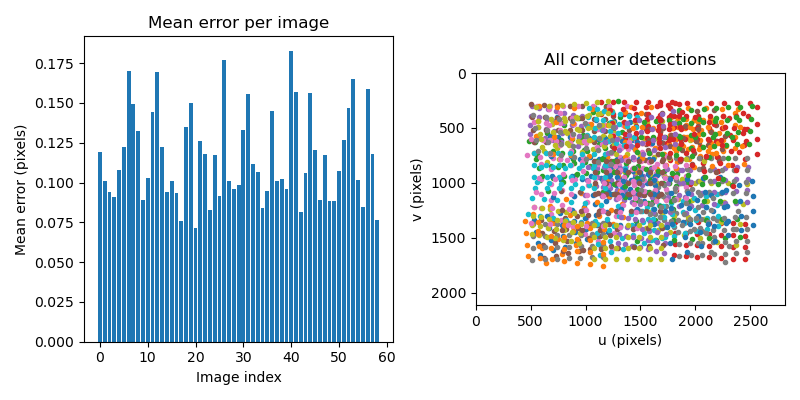
\includegraphics[width= \linewidth]{calibrationResult}
        \caption{Results of the camera calibration}
    \end{figure}

    \begin{description}
        \item [a)] There are several potential reasons that would result in significantly higher errors.
                This could be due to a strong tilt that often times also comes with changes of illumination.
                The visual tilting effect can also occur if the checkerboard is at the edge of the camera frame even though it is parallel to the image plane.
                To test this one could take a subset of pictures with a high visual tilting and calculate the error.
                If it applies there should be a significant difference to the error of the whole set.
        \item [b)] In general the accuracy looks quite alright.
                Whereas you can notice that it gets worse the closer you get to a corner.
                There you can still observe some distortion. 
                So if you were to extend the calibration picture database, it should be with pictures close to the image frame and especially the corners.
    \end{description}

    \subsection*{Task 1.2}

\section{Model creation}

    \subsection*{Task 2.1}
    \begin{description}
        \item [a)]  \hfill \\
            \begin{figure}[H]
                \center
                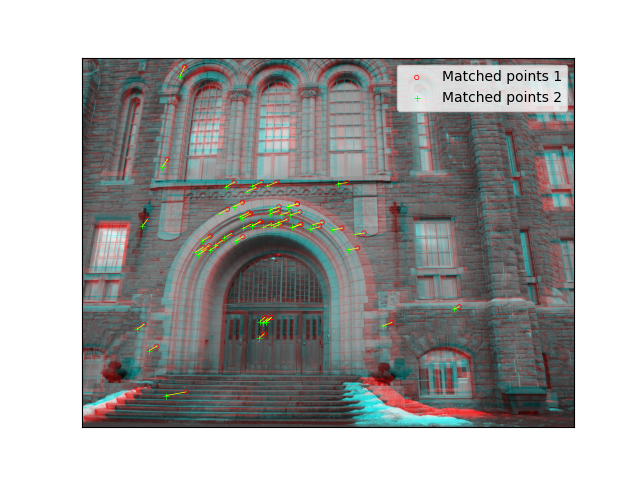
\includegraphics[width= 0.7\linewidth]{Correspondence}
                \caption{Best 50 correspondences by descriptor distance.}
            \end{figure}
            \begin{figure}[H]
                \center
                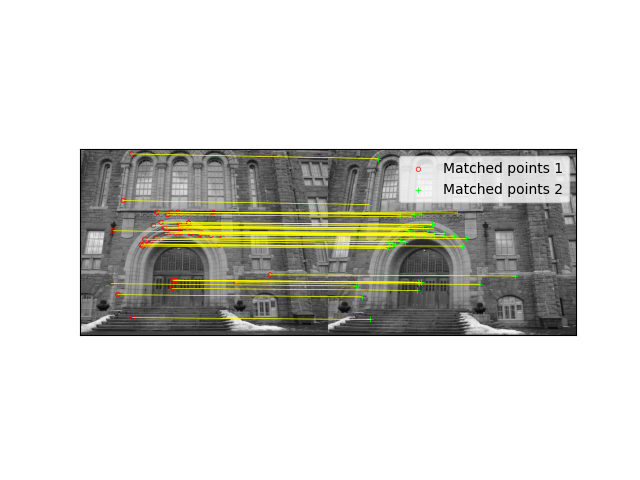
\includegraphics[width= \linewidth]{Matches}
                \caption{50 matches side by side.}
                \end{figure}
        \item [b)]  \hfill \\
            \begin{figure}[H]
                \center
                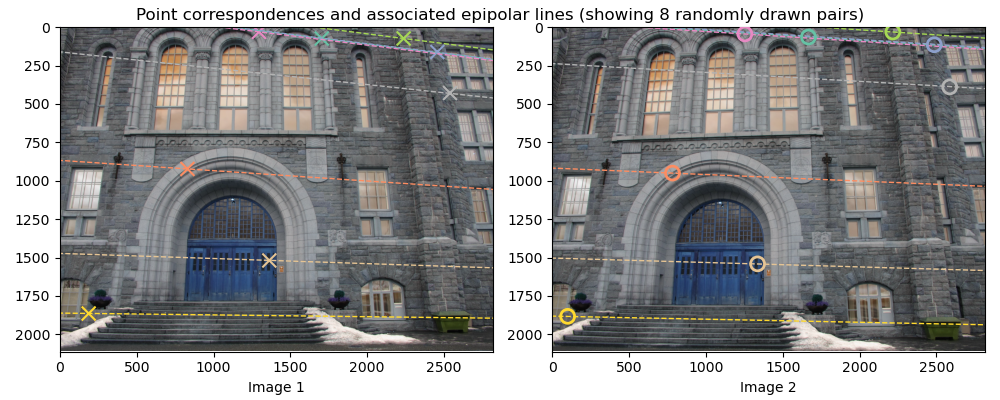
\includegraphics[width= \linewidth]{epipolarLines}
                \caption{8 inlier correspondences with their epipolar lines.}
            \end{figure}
        \item [c)]  In the included figures we used a maximum ratio og 0.9 and set the uniqueness parameter to true.
                    By playing around with these parameters we found that decreasing the max ratio results in way fewer matches, it also minimizes wrong matches.
                    Beside of the already pre-implemented knn distance metric we also tried out an ORB detector using the Hamming distance (commented out).
        \item [d)]  For estimating the relative pose and the 3D point coordinates we simply reused the RANSAC approach from HW5.
                    This gave us a total of 10966 inliers out of 12191 matches.
                    In the following figure you can see the pointcloud of the best solution.
            \begin{figure}[h]
                \center
                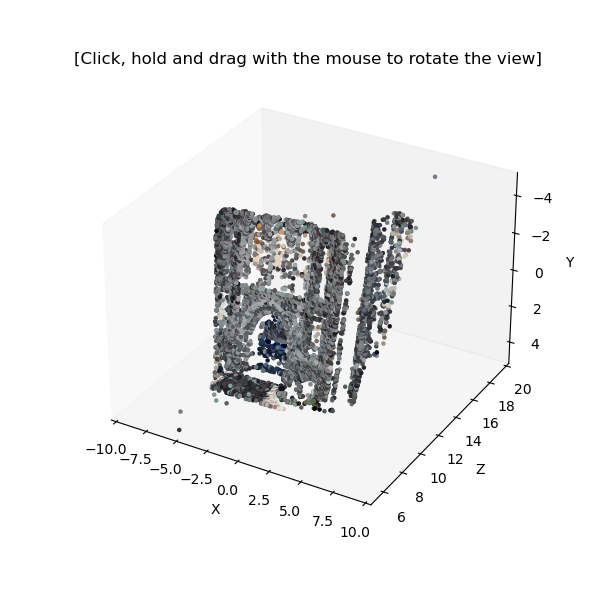
\includegraphics[width= 0.7 \linewidth ]{3D_point_cloud}
                \caption{Reconstructed 3D point cloud.}
            \end{figure}
        \item [e)]  The above point cloud consists of 10964 visible of 10966 total inlieres what is the pest found solution.
                    These reconstructions have been saved for later usage together with their correspondent feature descriptors.

    \end{description}
    
\end{document}